\documentclass[a4paper,12pt]{article}

\usepackage[utf8]{inputenc}
\usepackage[russian]{babel}
\usepackage{amsmath}
\usepackage{amssymb}
\usepackage{graphicx}

\title{Лекция 1 \\ Основы теории кодирования}
\date{}

\begin{document}

\maketitle

\section{Теорема Шеннона о кодировании}

Теорема кодирования Шеннона для канала с шумом определяет фундаментальный предел
надежной передачи данных по каналу связи, в котором присутствуют помехи.

Пусть дискретный канал связи имеет пропускную способность $C$, а источник сообщений
характеризуется энтропией $H$. Если скорость передачи информации $R$ меньше
пропускной способности канала ($R < C$), то существуют такие методы кодирования,
которые позволяют сделать вероятность ошибки декодирования сколь угодно малой.

С другой стороны, если скорость передачи превышает пропускную способность канала
($R > C$), то обеспечить надежную передачу информации невозможно.

Эта теорема является одной из основ теории информации и стала стимулом для развития
методов помехоустойчивого кодирования.

\section{Схема цифровой системы связи}

Типичная система цифровой связи включает следующие элементы:

\begin{center}
Источник $\rightarrow$ Кодер $\rightarrow$ Канал $\rightarrow$ Декодер $\rightarrow$ Приемник
\end{center}

\begin{figure}[h]
\centering
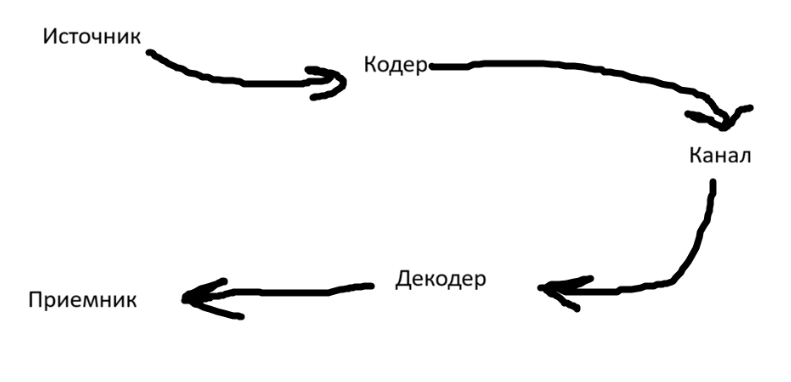
\includegraphics[width=0.8\textwidth]{images/communication_scheme.png}
\caption{Обобщенная схема цифровой системы связи}
\end{figure}

Источник формирует сообщение, которое может быть как непрерывным (например, речь),
так и дискретным (например, текст или цифровое изображение).

Кодер выполняет два типа преобразований:

\begin{itemize}
\item \textbf{Кодирование источника} — уменьшение избыточности исходных данных
(сжатие).
\item \textbf{Канальное кодирование} — добавление контролируемой избыточности,
позволяющей обнаруживать и исправлять ошибки.
\end{itemize}

После кодирования формируется последовательность символов, готовая к передаче
по каналу связи.

Канал представляет собой физическую среду передачи сигнала. Это может быть
радиоканал, оптоволокно или проводная линия связи.
Во время передачи сигнал подвергается воздействию шума, помех и затухания.

Декодер выполняет обратные операции: на основе принятого сигнала он
восстанавливает кодовое слово и затем извлекает исходное сообщение.

Приемник интерпретирует полученные данные и использует их по назначению,
например выводит звук через динамик или отображает изображение на экране.

\section{Двоичный симметричный канал}

Одной из наиболее простых моделей канала с ошибками является
\textbf{двоичный симметричный канал (Binary Symmetric Channel, BSC)}.

\begin{figure}[h]
\centering
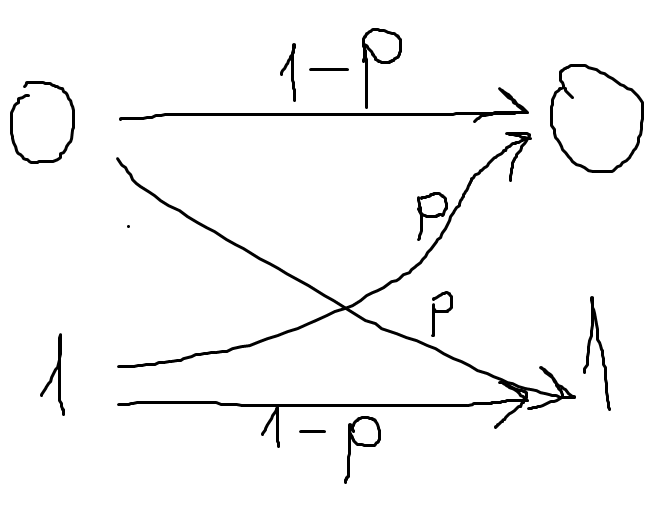
\includegraphics[width=0.6\textwidth]{./images/bsc_model.png}
\caption{Модель двоичного симметричного канала}
\end{figure}

В этой модели используются символы двоичного алфавита $\{0,1\}$.
Каждый переданный символ может быть принят правильно или с ошибкой.

Пусть $p$ — вероятность ошибки. Тогда:

\begin{itemize}
\item символ $0$ может быть принят как $1$ с вероятностью $p$,
\item символ $1$ может быть принят как $0$ с вероятностью $p$,
\item правильная передача происходит с вероятностью $1-p$.
\end{itemize}

Данный канал часто применяется в теоретических исследованиях,
поскольку его свойства симметричны и стационарны.

\section{Типы кодов}

Коды, предназначенные для защиты информации от ошибок,
можно разделить на несколько категорий.

\subsection{Блоковые коды}

В блоковых кодах поток данных разбивается на блоки длины $k$.
Каждый блок преобразуется в кодовое слово длины $n$, где $n > k$.

Дополнительные $(n-k)$ символов содержат избыточную информацию,
которая используется для обнаружения и исправления ошибок.

Кодирование каждого блока выполняется независимо от других.

\subsection{Сверточные коды}

В отличие от блоковых кодов, сверточные коды обрабатывают данные
как непрерывную последовательность.

Выходные символы зависят не только от текущих входных данных,
но и от нескольких предыдущих символов. Это достигается благодаря
наличию памяти в кодере.

Такой подход позволяет повысить эффективность кодирования,
однако усложняет процедуру декодирования.

\section{Метрики Хэмминга}

Для анализа свойств кодов используются характеристики,
введенные Ричардом Хэммингом.

\subsection{Вес Хэмминга}

Вес Хэмминга двоичного вектора $v$ определяется как количество
единичных элементов в этом векторе:

\[
w(v)
\]

Иными словами, это число единиц в двоичной последовательности.

\subsection{Расстояние Хэмминга}

Расстояние Хэмминга между двумя векторами $u$ и $v$
равно числу позиций, в которых они различаются:

\[
d(u,v)
\]

Для двоичных векторов это расстояние можно выразить через
операцию XOR:

\[
d(u,v) = w(u \oplus v)
\]

\section{Минимальное расстояние кода}

Важной характеристикой блокового кода является
\textbf{минимальное расстояние} $d_{min}$.

Оно определяется как минимальное расстояние Хэмминга
между двумя различными кодовыми словами.

Минимальное расстояние определяет способность кода
исправлять ошибки.

Код гарантированно исправляет до $t$ ошибок, если выполняется условие

\[
t \le \left\lfloor \frac{d-1}{2} \right\rfloor
\]

где $\lfloor x \rfloor$ обозначает целую часть числа.

Геометрически это означает, что вокруг каждого кодового слова
можно построить ``шар'' радиуса $t$, и такие шары не будут
пересекаться. Поэтому искаженное слово однозначно
соответствует исходному кодовому слову.

\section{Линейные коды}

Особый класс блоковых кодов — \textbf{линейные коды}.

В линейном двоичном коде длины $n$ множество кодовых слов
образует линейное подпространство размерности $k$
векторного пространства $F_2^n$.

\subsection{Порождающая матрица}

Линейный код можно задать с помощью
\textbf{порождающей матрицы} $G$ размера $k \times n$.

Ее строки образуют базис пространства кодовых слов.

Любое кодовое слово $c$ вычисляется по формуле

\[
c = uG
\]

где $u$ — информационный вектор длины $k$.

\subsection{Проверочная матрица}

Альтернативным способом описания кода является
использование \textbf{проверочной матрицы} $H$
размера $(n-k) \times n$.

Для любого кодового слова выполняется условие

\[
cH^T = 0
\]

или эквивалентная запись

\[
Hc^T = 0
\]

\subsection{Синдром}

Для принятого слова $r$ вычисляется синдром

\[
s = rH^T
\]

По значению синдрома можно определить наличие
и расположение ошибки.

Если строку проверочной матрицы обозначить
$h = (h_1, h_2, ..., h_n)$, то для любого
кодового слова $c = (c_1,...,c_n)$ выполняется

\[
\sum_{i=1}^{n} c_i h_i = 0
\]

в поле $F_2$.

Это означает, что кодовые слова ортогональны
каждой строке проверочной матрицы.

Связь между порождающей и проверочной матрицами
выражается соотношением

\[
GH^T = 0
\]

которое отражает ортогональность соответствующих
подпространств.

\end{document}